\chapter{Introducción al problema del clustering}\label{ch:clustering}

Para poder entender adecuadamente los algoritmos que han sido usados en ese trabajo, así como el tipo de problemas a los que se han aplicado, es necesario introducir una serie de conceptos teóricos. Comenzaremos explicando en este capítulo el problema del clustering clásico. 

\section{Introducción}

El problema de la agrupación o \emph{clustering} es un problema de aprendizaje no supervisado que consiste, como su propio nombre indica, en agrupar un conjunto de objetos, puntos, datos o items según una serie de características que tengan en común, de forma que los objetos que formen parte de un mismo \emph{cluster} sean de alguna forma similares entre sí, y que al mismo tiempo sean distintos de los que formen parte de clusters ajenos. Podemos entender, por tanto, que el clustering no es más que una forma de clasificar objetos.

El clustering y la clasificación en general son útiles para mantener un sumario que organice un conjunto de datos de gran tamaño, lo que permite un entendimiento más fácil y eficiente de la información contenida en él. Los primeros intentos de uso de métodos numéricos para la agrupación sistemática de objetos tuvieron lugar en las ciencias naturales, tales como la biología y la zoología, con el fin de obtener clasificaciones más objetivas y estables que permitiesen prescindir de la subjetividad de las técnicas tradicionales de taxonomía. Estas técnicas numéricas de agrupación han recibido distintos nombres según el campo en el que se han usado: \emph{taxonomía numérica} en biología, \emph{segmentación} en investigación de mercados, a veces \emph{Q-análisis} en psicología... En general, \emph{análisis de cluster} o simplemente \emph{clustering} quizá sean los términos genéricos con mayor aceptación. \cite{everitt2011cluster}

\section{Ejemplos de uso}

En \cite{everitt2011cluster} podemos encontrar algunos ejemplos de aplicación del clustering:
\begin{itemize}
	\item \textbf{Investigación de mercados}: clasificación de compañías según características financieras; clasificación de ciudades según tamaño, renta per cápita, etc \cite{green1967cluster}, clasificación de clientes para encontrar compradores potenciales de un cierto producto \cite{chakrapani2004statistics}.
	\item \textbf{Astronomía}: clasificación de nebulosas según composición química \cite{faundez1996classification}, clasificación de estrellas según su velocidad hacia el centro de la galaxia y su velocidad de rotación alrededor de la galaxia \cite{celeux1992classification}.
	\item \textbf{Arqueología}: creación de una taxonomía de hachas encontradas en las islas británicas según tamaño y tipo de punta \cite{hodson1971numerical}, análisis de coprolitos para estudiar el maíz presente en la alimentación \cite{sutton1995cluster}.
	\item \textbf{Bioinformática y genética}: uso de clustering en datos genéticos para identificar tipos de cáncer asociados a una mayor probabilidad de supervivencia \cite{eisen1998cluster}.
\end{itemize}


\begin{figure}
	\centering
	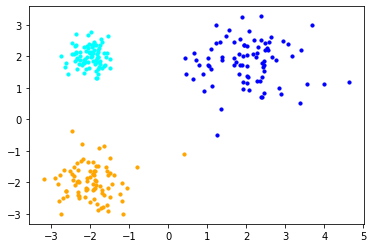
\includegraphics[width=0.7\textwidth]{Images/clusters}
	\caption{Ejemplo de tres clusters claramente distinguibles y separables con densidades distintas.}
	\label{fig:clusters}
\end{figure}



\section{Definiciones formales}

Hasta ahora, se ha dado una interpretación bastante intuitiva acerca de en qué consiste el clustering. Llega el momento de definir formalmente el problema del clustering e introducir su notación. Para tal fin, en toda esta sección nos basaremos en el trabajo realizado en \cite{jose2016automatic}.

\subsection{Notación}

Los siguientes son elementos típicos de un problema de clustering:

\begin{itemize}
	\item Un \emph{objeto}, \emph{patrón} o \emph{instancia} es un dato individual representado por un vector $\textbf{x} = (x_1, x_2,\dots, x_D )^T$, donde $x_i \in \mathbb{R}$ es una \emph{característica} o atributo, y $D$ representa la \emph{dimensionalidad} (el número de características que tienen los objetos). 
	\item Un \emph{conjunto de datos} (o \emph{dataset} en inglés) es una matriz\newline$\textbf{X} = ( \textbf{x}_1, \textbf{x}_2, \dots, \textbf{x}_N )$, donde $\textbf{x}_i \in \mathbb{R}^{D}$ para $i=1,\dots,N$, y $N$ es el número total de objetos en el conjunto de datos.
	\item Un \emph{cluster} puede definirse como una región del espacio que contiene objetos.
	\item Una \emph{solución de clustering} $\textbf{C} = \{c_k | k=1,\dots,K \}$ es un conjunto de clusters disjuntos que particiona al conjunto de datos $\textbf{X}$ en $K$ grupos.
	\item El número de objetos en el cluster $\textbf{c}_k$ es el valor expresado como $n_k = |\textbf{c}_k|$
	\item El \emph{centroide} o \emph{prototipo} del cluster $\textbf{c}_k$ (o prototipo de $\textbf{c}_k$) se expresa como $\textbf{\=c}_k = \frac{1}{n_k}\sum_{\textbf{x}_i \in \textbf{c}_k} \textbf{x}_i$.
	\item El centroide del conjunto de datos \textbf{X} o \emph{centroide global} de \textbf{X} es\newline$\textbf{\=X} = \frac{1}{N} \sum_{\textbf{x}_i \in \textbf{X}} \textbf{x}_i$
	\item Una \emph{medida de distancia} es una métrica usada para cuantificar la proximidad (cercanía o lejanía) entre objetos.
	\item Un \emph{índice de validez} o CVI (\emph{cluster validity index}) usa una medida de distancia para evaluar cuantitativamente una solución de clustering obtenida.
\end{itemize}
\subsection{Tipos de algoritmos de clustering}

El clustering no es un algoritmo en sí, sino el tipo de problema que se pretende resolver, para el cual pueden usarse diferentes técnicas. Tradicionalmente, se han considerado dos tipos de algoritmos para el problema del clustering:

\begin{itemize}
	\item \textbf{Algoritmos de clustering parcicional}: estos algoritmos dividen directamente el conjunto de datos en un determinado número de clusters. De esta forma, un conjunto de datos $\textbf{X}$ es particionado en $K$ grupos (o clusters) disjuntos $\textbf{C} = \{ \textbf{c}_{1},\textbf{c}_{2},\dots,\textbf{c}_{K}\}$, de forma que se cumplan tres condiciones:
	\begin{enumerate}
		\item No puede haber clusters vacíos: $\textbf{c}_i \neq \emptyset,~~~i=1,\dots,K$.
		\item La unión de todos los clusters es igual al conjunto de datos: $\bigcup_{i=1}^{K}\textbf{c}_i =  \textbf{X}$.
		\item Los clusters son disjuntos, es decir, no hay solapamientos: $\textbf{c}_i \cap \textbf{c}_j = \emptyset,~~~~i,j=1,\dots,K~~~ \text{y además} ~~~i \neq j$.
		
		
	\end{enumerate}
	
	El algoritmo de clustering particional más conocido probablemente sea el $k$-means \cite{macqueen1967some}, que funciona asignando cada objeto al cluster cuyo centroide se encuentre más cerca, para posteriormente recalcular los centroides como los promedios de los objetos asociados a los respectivos clusters, de forma que las distancias entre los objetos y los centroides de los clusters a los que están asignados se minimizan.
	
	\item \textbf{Algoritmos de clustering jerárquico}: los algoritmos de este tipo producen como salida una jerarquía de clusters llamada \emph{dendograma}, que representa las agrupaciones anidades de los objetos. Al crear un dendograma, se generan $N$ niveles de clustering, de manera que cada nivel se construye a partir del anterior. De esta forma, no es necesario establecer un número de clusters a priori, puesto que en cada nivel se generan distintos números de clusters. Los dos métodos principales de clustering jerárquico son el aglomerativo y el divisivo.
\end{itemize}




\subsection{Índices de validación}\label{subsct:cvi}

Un índice de validación o CVI (\emph{cluster validity index}) evalúa cómo de buena es una solución (partición) de clustering que ha sido generada por un algoritmo, usando únicamente información inherente al conjunto de datos (es decir, sin tener conocimiento de cuál es la solución óptima, puesto que en aprendizaje no supervisado, en principio, no se sabe cuál es). Un buen índice de validación debería tener un significado intuitivo, debería ser fácil de calcular y debería ser justificable matemáticamente, además de que debería permitir establecer un orden entre las soluciones obtenidas según cómo de buenas son.

Dependiendo del índice que se vaya a emplear para evaluar soluciones, habrá que buscar la solución que maximice o minimice el índice escogido. Por tanto, podemos distinguir entre índices de maximización e índices de minimización.

Son numerosos los índices de validez existentes. A continuación, se listan algunos de los más utilizados:

\begin{itemize}
	\item \textbf{Dispersión intra-grupo} (\emph{within-group scatter}, WGS) \cite{macqueen1967some}. Índice de minimización, también llamado dispersión intra-cluster. Mide la suma de distancias (euclídeas) al cuadrado entre los objetos y los centroides de los clusters a los que pertenecen:
	
	\begin{equation}
		\text{WGS}(\textbf{C}) = \sum_{\textbf{c}_k \in \textbf{C}} \sum_{\textbf{x}_i \in \textbf{c}_k} \text{d}_{\text{e}}^2 (\textbf{x}_i,\textbf{\=c}_k),
	\end{equation}
	
	donde $\text{d}_{\text{e}}(\dots)$ representa la métrica de distancia euclídea entre dos puntos:
	
	\begin{equation}\text{d}_{\text{e}}(\textbf{a},\textbf{b}) = \sqrt{\sum_{i=1}^{n}{(a_i-b_i)^2}}.
	\end{equation}
	

	\item \textbf{Dispersión entre grupos} (\emph{between-group scatter}, BGS) \cite{theodoridis1999pattern}. Índice de maximización. Mide la suma de distancias entre los centroides de los clusters:
	
	\begin{equation}
		\text{BGS}(\textbf{C}) = \sum_{\textbf{c}_k,\textbf{c}_r \in \textbf{C}} \text{d}_{\text{e}} (\textbf{\=c}_k,\textbf{\=c}_r).
	\end{equation}
	
	\item \textbf{Índice de conectividad} (\emph{connectivity index}) \cite{handl2007evolutionary}. Índice de minimización. Mide el grado en el que objetos vecinos han sido asignados al mismo cluster:
	
	\begin{equation}\label{eq:conn}
		\text{Conn}(\textbf{C}) = \sum^{N}_{i=1}\left( \sum^{L}_{j=1} a_{i,n_{ij}} \right),
	\end{equation}
	
	donde
	
	\begin{equation}
	a_{i,n_{ij}} = \begin{cases}
       \frac{1}{j} &\quad\text{si  } \neg \exists \textbf{c}_k : \textbf{x}_i \in \textbf{c}_k \land \textbf{x}_{n_{ij}} \in \textbf{c}_k\\
       0 & \quad\text{en caso contrario}\\
  	\end{cases},
  \end{equation}
	
	donde $n_{ij}$ hace referencia al $j$-ésimo vecino más cercano del $i$-ésimo objeto. Por su parte, $L$ es un parámetro que establece el número de vecinos a tener en cuenta al calcular el índice de conectividad.
	
	Intuitivamente, lo que hace este índice es añadir una penalización cada vez que se detectan objetos vecinos (cercanos) pertenecientes a clusters distintos.
	
	\item \textbf{Índice Calinski-Harabasz} (CH) \cite{calinski1974dendrite}. Índice de maximización. Calinski-Harabasz ofrece una proporción entre la separación y la cohesión  de los clusters. La cohesión se estima como la suma de las distancias entre los objetos y sus respectivos centroides, y la separación se mide como la distancia entre los centroides de los clusters y el centroide global de todo el conjunto de datos:
	
	\begin{equation}
		\text{CH}(\textbf{C}) = \frac{N-K}{K-1} \times \frac{\sum_{\textbf{c}_k \in \textbf{C}} n_k \text{d}_{\text{e}}(\textbf{\=c}_k, \textbf{\=X})}{\sum_{\textbf{c}_k \in \textbf{C}} \sum_{\textbf{x}_i \in \textbf{c}_k} \text{d}_{\text{e}}(\textbf{x}_i, \textbf{\=c}_k)}.
	\end{equation}
	
	\item \textbf{Índice Davies-Bouldin} (DB) \cite{davies1979cluster}. Índice de minimización. En este caso, la cohesión es estimada con la distancia media entre los objetos y sus respectivos centroides, y la separación se calcula con la distancia entre centroides:
	
	\begin{equation}\label{eq:db}
		\text{S}(\textbf{C}) = \frac{1}{K} \sum_{\textbf{c}_k \in \textbf{C}} \max_{\textbf{c}_r \in \textbf{C} \setminus \textbf{c}_k} \left\{\frac{\text{S}(\textbf{c}_k) + \text{S}(\textbf{c}_r)}{\text{d}_{\text{e}}(\textbf{\=c}_k,\textbf{\=c}_r)}\right\},
	\end{equation}
	
	donde
	
	\begin{equation}
	\text{S}(\textbf{c}_k) = \frac{1}{n_k} \sum_{\textbf{x}_i \in \textbf{c}_k} \text{d}_\text{e}(\textbf{x}_i,\textbf{\=c}_k).
	\end{equation}
	
	\item \textbf{Índice Silhouette} (SI) \cite{rousseeuw1987silhouettes}. Índice de maximización. Se trata de una sumatoria normalizada, en en la cual la cohesión se calcula como la suma de las distancias entre los puntos pertenecientes a un mismo cluster, y la separación se basa en la distancia entre los puntos más cercanos pertenecientes a clusters distintos:
	
	\begin{equation}
		\text{SI}(\textbf{C}) = \frac{1}{N} \sum_{\textbf{c}_k \in \textbf{C}} \sum_{\textbf{x}_i \in \textbf{c}_k}
		\frac{\text{b}(\textbf{x}_i,\textbf{c}_k) - \text{a}(\textbf{x}_i,\textbf{c}_k)}{\max\{\text{b}(\textbf{x}_i,\textbf{c}_k),\text{a}(\textbf{x}_i,\textbf{c}_k)\}},
	\end{equation}
	
	donde:
	
	\begin{equation}\text{a}(\textbf{x}_i,\textbf{c}_k) = \frac{1}{n_k} \sum_{\textbf{x}_j \in \textbf{c}_k} \text{d}_{\text{e}}(\textbf{x}_i,\textbf{x}_j),
	\end{equation}
	
	\begin{equation}
	\text{b}(\textbf{x}_i,\textbf{c}_k) = \min_{\textbf{c}_r \in \textbf{C} \setminus \textbf{c}_k} \left\{ \sum_{\textbf{x}_j \in \textbf{c}_r} \text{d}_{\text{e}}(\textbf{x}_i,\textbf{x}_j) \right\}.
	\end{equation}
\end{itemize}
	

\subsection{Clustering como problema de optimización}\label{subsct:optclust}

El problema del clustering puede formularse como un problema de optimización.

Sea $\Omega$ el conjunto de todas las posibles soluciones de clustering (particiones) para un conjunto de datos $\textbf{X}$ dado, y sea $f$ una función objetivo, que puede ser cualquiera de los índices de validez presentados en la sección \ref{subsct:cvi}. Suponiendo que se ha optado por utilizar un índice de validez de minimización, entonces el objetivo del problema de clustering $(\Omega,f)$ consiste en encontrar la solución de clustering óptima $\textbf{C}^{*}$, para la cual

\begin{equation}
	f(\textbf{C}^{*}) = \min\{ f(\textbf{C}) | \textbf{C} \in \Omega \}.
\end{equation}


% ¿Ejemplos uso clustering?
